% simdoc.tex V3.0, 30 March 2010

\documentclass[12pt, times]{simauth}

\usepackage{moreverb}

%\usepackage[T1,mtbold]{mathtime} % commented by ShareLaTeX Team because of compilation errors

\usepackage[
%dvips, % commented by ShareLaTeX Team because of compilation errors
colorlinks,bookmarksopen,bookmarksnumbered,citecolor=red,urlcolor=red]{hyperref}

\usepackage[utf8]{inputenc}
\usepackage[T1]{fontenc}
\usepackage[spanish]{babel}
\usepackage{upquote}
\usepackage{epigraph}
\usepackage{makeidx}
\usepackage{framed}
\usepackage{pgf}
\usepackage{tikz}
\usepackage{amsmath,cases,mathtools}
\usepackage{amsthm}
\usepackage{array}
\usepackage{MnSymbol,wasysym}
\usepackage[pdftex,active,tightpage]{preview}
\usetikzlibrary{babel}
\usetikzlibrary{arrows,automata,positioning}
\graphicspath{ {imagenes/} }
\usepackage{pgfplots}
\usepackage[lined,boxed,commentsnumbered]{algorithm2e}
\usepackage{calligra}
\usetikzlibrary{er}


\def\volumeyear{2010}

\SetKwProg{Fn}{Function}{}{}

\begin{document}

%\runninghead{A.~N.~Other}

\title{
    {\fontfamily{ppl} \fontsize{30}{1} \selectfont{
        Tarea 2: Tiempo Lógico }
    }
}

\author{
    {\fontfamily{ppl} \fontsize{14}{1} \selectfont{
        Carlos Martín Flores González \\
        Carné: 2015183528\\ 
        17 de Abril del 2017
        }
    }
}

%\address{John Wiley \& Sons, Ltd, The Atrium, Southern Gate, Chichester,
%West Sussex, PO19~8SQ, UK}
%
%\corraddr{Journals Production Department, John Wiley \& Sons, Ltd,
%The Atrium, Southern Gate, Chichester, West Sussex, PO19~8SQ, UK.}

%\begin{abstract}
%This paper describes the use of the \LaTeXe\ \textsf{simauth.cls}
%class file for setting papers for \emph{Statistics in Medicine}.
%\end{abstract}

%\keywords{class file; \LaTeXe; \emph{Statist.\ Med.}}

\maketitle

\tableofcontents

\section{Demuestre matemáticamente la propiedad fuerte del reloj para relojes vectoriales.}

De acuerdo con \cite{fidge} para mantener orden parcial, en lugar de utilizar un solo valor entero (como se propone en \cite{lamport}, las marcas de tiempo son representadas por medio de un arreglo $[c_1, c_2 \dots c_n]$ con un valor de reloj entero para cada proceso en la red. Se usa $e_p$ para representar un evento $e$ en un proceso $p$, y $T_{e_p}$ el arreglo de marcas de tiempo (\emph{timestamp arrays}) ligado al registro permanente de la ejecución de este evento. 

Estos arreglos de marcas de tiempo se mantienen con las siguientes reglas:
\begin{itemize}
    \item[] \textbf{Regla RA1:} Todos los valores iniciales son cero.
    \item[] \textbf{Regla RA2:} El valor de reloj local se incrementa al menos una vez antes de cada evento atómico.
    \item[] \textbf{Regla RA3:} El valor actual del arreglo de marcas de tiempo es acarreado en cada señal saliente.
    \item[] \textbf{Regla RA4:} Al recibir una señal, un proceso pone en el valor de cada entrada del arreglo de marcas de tiempo el máximo de dos valores correspondientes en el arreglo local y en el arreglo acarreado que fue recibido.
    \item[] \textbf{Regla RA5:} Los valores en los arreglos de marcas de tiempo nunca son decrementados.
\end{itemize}

Marcas de tiempo ligadas a registros almacenados de eventos son comparados de la siguiente forma:
\begin{equation}
    \tag{EA1}
    e_p \to f_p \textnormal{\textbf{ iff }} T_{e_p}[p] < T_{f_q}[p]
\end{equation}

En esencia esto dice que un evento $e_p$ tiene que haber ocurrido antes del evento $f_q$ si y sólo si el proceso $q$ ha recibido una señal desde $p$ (ya sea directa o indirectamente) que fue enviada después, o en el mismo momento, de la ejecución de $e_p$.


\subsection{$V(a) < V(b) \Longleftrightarrow a \to b$} \label{primeprueba}
\cite{lamport} define $\to$ para el caso asincrónico como: ``la relación más pequeña que satisface las siguientes tres condiciones: (i) Si $a$ y $b$ son eventos en el mismo proceso, y $a$ viene antes de $b$, entonces $a \to b$. (ii) Si $a$ es el envío de un mensaje de un proceso y $b$ es el receptor del mensaje en otro proceso, entonces $a \to b$. (iii) Si $a \to b$ y $b \to c$ entonces $a \to c$''

\noindent \paragraph{}(i) Sea ambos $a$ y $b$ eventos que pertenecen al mismo proceso $r$, y $a$ ocurre antes de $b$. Asumir: 
\begin{equation}
a_r \to b_r
\end{equation}
Entonces por definición \textbf{EA1} 
\begin{equation} \label{eq:2}
T_{a_r}[r] < T_{b_r}[r]
\end{equation}
La cual es verdadera por las reglas \textbf{RA2} y \textbf{RA5}.


\noindent \paragraph{} (ii) Sea $a_r$ una señal de envío y $b_s$ la recepción de la misma señal. Asumir:
\begin{equation}
    a_r \to b_s
\end{equation}

Entonces por \textbf{EA1}
\begin{equation}
T_{a_r}[r] < T_{b_s}[r]
\end{equation}

Ahora, asumir que $b_{\overline{s}}$ es el evento en el proceso $s$ que precede inmediatamente a $b_s$. Entonces por regla \textbf{RA4}
\begin{equation}\label{eq:5}
T_{a_r}[r] < (\textnormal{\textbf{if }} T_{b_{\overline{s}}} \leq T_{a_r}[r] \textnormal{\textbf{ then }} T_{a_r}[r] + 1 \textnormal{\textbf{ else }} T_{b_{\overline{s}}}[r])
\end{equation}

La expresión a la derecha de \ref{eq:5} implica que
\begin{equation}
(T_{b_{\overline{s}}}[r] \leq T_{a_r}[r] \land T_{a_r}[r] < T_{a_r}[r] + 1) \lor (T_{b_{\overline{s}}}[r] > T_{a_r}[r] \land T_{b_{\overline{s}}}[r] > T_{a_r}[r])
\end{equation}

Lo que se reduce a
\begin{equation}
(T_{b_{\overline{s}}}[r] \leq T_{a_r}[r]) \lor (T_{b_{\overline{s}}}[r] > T_{a_r}[r])
\end{equation}

Lo cual debe ser verdadero.

\subsection{$V(b) < V(a) \Longleftrightarrow b \to a$}
En este caso el evento $b$ inició antes que el $a$, por lo que para probar su correctitud tiene que cumplir con las propiedades expuestas en \ref{primeprueba}. 

\subsection{$V(a) = V(b) \Longleftrightarrow a = b$}
\begin{proof}[Prueba]
Suponer que $V(a) = V(b) \Longleftrightarrow a \ne b$. Si $V(a) = V(b)$ entonces hay un $k$ tal que
\begin{align*}
V(a) = k\\
V(b) = k 
\end{align*}

Pero se sabe por \textbf{RA2} que el reloj local se incrementa al menos una vez antes de cada evento atómico, y si $a$ y $b$ son diferentes entonces debería de existir una diferencia entre los valores de $V(a)$ y $V(b)$, pero ambos devuelven $k$ lo que significa que los eventos $a$ y $b$  el reloj no experimentó cambios. Contradicción, $a$ y $b$ son el mismo evento.
\end{proof}

\subsection{$V(b) \parallel V(a) \Longleftrightarrow a \parallel b$}
\begin{proof}[Prueba]
(1) Suponer $V(b) \parallel V(a) \Rightarrow a \to b$. Si $V(b) \parallel V(a)$ quiere decir que hay dos vectores $U$ y $W$ tal que:
\begin{align*}
V(b) = U\\
V(a) = W 
\end{align*}

Se sabe por definición de $U \parallel W$ que $\{\exists i,j$ $|$ $U[i] < W[i], U[j] > W[j]\}$. Si $U \parallel W$ entonces en algún punto $U > W$ y al darse esta condición, la definición \textbf{EA1} no se da la cual es necesaria para argumentar que $a \to b$ . Contradicción, $V(b) \parallel V(a) \nRightarrow a \to b$ 

\paragraph{} (2) Suponer $V(b) \parallel V(a) \Rightarrow b \to a$. Si $V(b) \parallel V(a)$ quiere decir que hay dos vectores $U$ y $W$ tal que:
\begin{align*}
V(b) = U\\
V(a) = W 
\end{align*}

Se sabe por definición de $U \parallel W$ que $\{\exists i,j$ $|$ $U[i] < W[i], U[j] > W[j]\}$. Si $U \parallel W$ entonces en algún punto $W > U$ y al darse esta condición, la definición \textbf{EA1} no se da la cual es necesaria para argumentar que $b \to a$ . Contradicción, $V(b) \parallel V(a) \nRightarrow b \to a$ 

\paragraph{}Si (1) $\land$ (2) se puede argumentar que $a \parallel b$ puesto a que tanto en (1) como en (2) se muestra que no hubo relación causal entre los eventos.

\end{proof}

La prueba anterior está inspirada en el teorema 10 expuesto en \cite{mattern} para decidir si dos eventos están causalmente relacionados o no. 

\paragraph{Teorema 10 (Mattern)} $\forall e, e' \in E: e < e' \text{ \emph{iff} } C(e) < C(e') \text{ \emph{and} } e \parallel e' \text{\emph{ iff }} C(e) \parallel C(e')$\\
Brinda un método simple para decidir si dos eventos $e, e'$ están causalmente relacionados o no: se toma las marcas de tiempo $C(e)$ y $C(e')$ y se verifica si $C(e) < C(e')$ o $C(e') < C(e')$. Si la prueba pasa, los eventos están causalmente relacionados. De otra forma son causalmente independientes.

\subsection{Trabajo relacionado}
Aunque no se expone como parte de esta tarea, el método utilizado por \cite{garg} para probar las propiedades del reloj vectorial me pareció muy elegante. Se utiliza inducción matemática y 
conjuntos para determinar posibles caminos entre eventos y de esa forma determinar si hay una relación causal de uno con respecto a otro. No incluí nada de esto en mi solución porque me quise ajustar al uso de reglas de relojes vectoriales para intentar probar la condición fuerte del reloj (aparte que para llegar a la demostración por inducción, \cite{garg} invierte bastante en el montaje del marco teórico que acompañaran a sus pruebas).  

\section{Dado un conjunto arbitrario de relojes vectoriales todos de las mismas dimensiones, podría haber uno o más relojes vectoriales que no pueden venir de la misma historia global que los otros. Dé al menos 2 ejemplos de conjuntos de relojes vectoriales con esta característica.}

En \cite{meneses} se propone el problema del conjunto de relojes vectoriales posibles e imposibles, en donde, dado un conjunto arbitrario, finito de relojes vectoriales, se debe encontrar una historia distribuida que contenga eventos marcados en tiempo con relojes vectoriales del conjunto. Se muestra que hay conjuntos imposibles para los cuales no hay una historia distribuida que los contiene. En su forma más general el problema puede ser definido como: 
\begin{center}
``Dado un conjunto de marcas de tiempo vectoriales (\emph{vector timestamps}), decidir si existe una historia distribuida o no que los contiene. No hay información disponible acerca del sitio donde cada reloj vectorial se supone que ha ocurrido.''
\end{center}

\paragraph{Teorema 1 (Meneses - Zona desierta):} Sean $a_1, a_2, \dots, a_n$ $n$ eventos en $\mathcal{H}$ asociados con $n$ relojes vectoriales $v_1, v_2, \dots, v_n$ respectivamente. Permitir también que los $n$ eventos sean concurrentes entre sí. Si $t = \text{\emph{maximum}}(v_1, v_2, \dots, v_n)$, entonces, no puede existir un evento \textbf{z} $\in \mathcal{H}$ tal que $v_i \to V(\text{\textbf{z}}) \to t$, para cualquier $i$.
La prueba de este teorema se proporciona en \cite{meneses}. 

\subsection{Ejemplo 1}
El conjunto de relojes vectoriales $\mathcal{B}$ es imposible:
\begin{align*}
\mathcal{B} = \{ & [\langle 2,0,1 \rangle, \text{\emph{site }} 1] \\
                  & [\langle 0,1,0 \rangle, \text{\emph{site }} 2] \\  
                  & [\langle 0,1,1 \rangle, \text{\emph{site }} 2] \\
                  & [\langle 1,3,2 \rangle, \text{\emph{site }} 2] \\
                  & [\langle 0,0,2 \rangle, \text{\emph{site }} 3] \} 
\end{align*}
Para probar que $\mathcal{B}$ es un conjunto imposible, se consideran los relojes vectoriales concurrentes $v_1 = \langle 0,1,0 \rangle$ y $v_2 = \langle 2,0,1 \rangle$, ambos en $\mathcal{B}$. Supongamos que estos relojes vectoriales corresponden a los eventos \textbf{a}$_1$ y \textbf{a}$_2$. Siguiendo el Teorema 1, si se computa el máximo entre $v_1$ y $v_2$, se obtiene $t = \langle 2,1,1 \rangle$. Entonces no puede existir un evento \textbf{z} en la misma historia distribuida que \textbf{a}$_1$ y \textbf{a}$_2$, tal que su reloj vectorial asociado $V(\text{\textbf{z}})$ tenga la propiedad: $v_1 < V(\text{\textbf{z}}) < t$ o $v_2 < V(\text{\textbf{z}}) < t$. Sin embargo, el reloj vectorial $\langle 0,1,1 \rangle$ en $\mathcal{B}$ está entre $\langle 0,0,1 \rangle$ y $t = \langle 2,1,1 \rangle$, lo que hace que el conjunto $\mathcal{B}$ sea imposible. En la figura \ref{fig:imposible1} se muestra una representación gráfica de esta situación particular.

\begin{figure}[h]
\centering
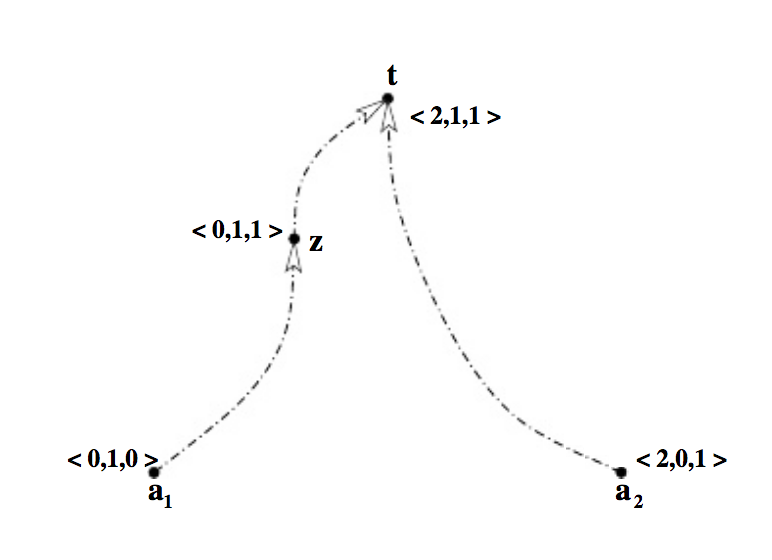
\includegraphics[width=0.5\textwidth]{conjunto-imposible-1}
\caption{Conjunto imposible debido al teorema de la zona desierta. Tomado de \cite{meneses}.}
\label{fig:imposible1}
\end{figure}


El conjunto de relojes vectoriales $\mathcal{B}$ es imposible:
\begin{align*}
\mathcal{B} = \{ & [\langle 2,0,1 \rangle, \text{\emph{site }} 1] \\
                  & [\langle 0,1,0 \rangle, \text{\emph{site }} 2] \\  
                  & [\langle 0,1,1 \rangle, \text{\emph{site }} 2] \\
                  & [\langle 1,3,2 \rangle, \text{\emph{site }} 2] \\
                  & [\langle 0,0,2 \rangle, \text{\emph{site }} 3] \} 
\end{align*}
Para probar que $\mathcal{B}$ es un conjunto imposible, se consideran los relojes vectoriales concurrentes $v_1 = \langle 0,1,0 \rangle$ y $v_2 = \langle 2,0,1 \rangle$, ambos en $\mathcal{B}$. Supongamos que estos relojes vectoriales corresponden a los eventos \textbf{a}$_1$ y \textbf{a}$_2$. Siguiendo el Teorema 1, si se computa el máximo entre $v_1$ y $v_2$, se obtiene $t = \langle 2,1,1 \rangle$. Entonces no puede existir un evento \textbf{z} en la misma historia distribuida que \textbf{a}$_1$ y \textbf{a}$_2$, tal que su reloj vectorial asociado $V(\text{\textbf{z}})$ tenga la propiedad: $v_1 < V(\text{\textbf{z}}) < t$ o $v_2 < V(\text{\textbf{z}}) < t$. Sin embargo, el reloj vectorial $\langle 0,1,1 \rangle$ en $\mathcal{B}$ está entre $\langle 0,1,0 \rangle$ y $t = \langle 2,1,1 \rangle$, lo que hace que el conjunto $\mathcal{B}$ sea imposible. En la figura \ref{fig:imposible1} se muestra una representación gráfica de esta situación particular.

\subsection{Ejemplo 2}
El conjunto $\mathcal{S} = \{\langle 100,0,100 \rangle, \langle 0, 100, 0\rangle, \langle 50,100,0 \rangle\}$ es imposible. Tomando como base el ejemplo anterior, si se toman los relojes vectoriales concurrentes $v_1 = \langle 100,0,100 \rangle$ y $v_2 = \langle 0,100,0 \rangle$ y se computa el máximo entre ambos se obtiene $t = \langle 100,100,100 \rangle$. Sin embargo, el reloj vectorial $\langle 50,100,0 \rangle$ está entre $\langle 0,100,0 \rangle$ y $\langle 100,100,100 \rangle$, lo que hace que $\mathcal{S}$ sea imposible.


%\setlength{\unitlength}{1mm}
%\begin{picture}(60,50)
%  \put(0 ,15){\vector(1,0){53}}  
%  \put(54,14){$x_A$}
%  \put( 8,10){\vector(0,1){37}} 
%  \put( 0,46){$ct_A$}
%  \multiput(13,9)(15,0){3}{\line(0,1){35}}   
%  \put(11,5){$A''$}
%  \put(26,5){$A'$}
%  \put(41,5){$A'''$}
%  \multiput(13,37)(30,0){2}{\circle*{2}}
%  \put(28,22){\circle*{2}}
%  \put(28,22){\vector(1,1){14}}  
%  \put(15,39){$E_1$}
%  \put(28,22){\vector(-1,1){14}} 
%  \put(45,39){$E_2$}
%  \multiput(0,37)(4,0){13}{\line(1,0){2}}
%\end{picture}


\section{Investigue la técnica conocida como ``relojes plausibles''. Explique su propósito, implementación y casos donde sos utilizables.}

\subsection{Propósito}
Los relojes pausibles son una clase de reloj lógico que puede ser implementado con una serie de componentes que no son afectados por el tamaño del sistema y aún así proporcionar buena precisión en el ordenamiento.

\paragraph{}Aunque los relojes vectoriales pueden ordenar eventos en un sistema distribuido de forma precisa y detectar eventos concurrentes, son costosos de mantener y manipular debido a que vectores de enteros deben ser incluidos en los mensajes y es necesario compararlos para determinar el orden entre las operaciones. Además, dado que los relojes vectoriales tienen un componente por cada nodo en el sistema, no son escalables. 

Los relojes vectoriales son útiles en la comprensión del comportamiento de sistemas distribuidos. Sin embargo, tienen una gran desventaja, no ser constantes en tamaño: la implementación de relojes vectoriales requieren una entrada para cada uno de los $N$ sitios en el sistema. Si $N$ es grande, muchos problemas pueden surgir. Hay costos crecientes el almacenamiento porque cada sitio debe reservar espacio para mantener la versión local del reloj vectorial y, dependiendo de un sistema en particular, los tiempos del vector asociados con ciertos eventos tienen también que ser almacenados. Todos los mensajes de una computación distribuida son etiquetados con marcas de tiempo leídas desde el reloj vectorial. También, la comparación de marcas de tiempo vectoriales para determinar el ordenamiento entre eventos va a tener alto \emph{overhead} de procesamiento para un $N$ grande. Por esto los relojes vectoriales tienen pobre escalabilidad.


\paragraph{}Los relojes escalares pueden ser implementados eficientemente (por ejemplo, los relojes de Lamport), pero cuando los eventos son marcados en el tiempo (\emph{timestamped}) con estos relojes, dos eventos pueden aparecer ordernados de acuerdo a sus marcas de tiempo incluso cuando son concurrentes. En un sistema de objetos distribuidos, esto puede llevar a operaciones de consistencia innecesarias. En 1978, Leslie Lamport propone el concepto de \emph{relojes lógicos} que definen el orden entre los eventos en sistemas distribuidos \cite{lamport}. Consiste de un mapeo $\tau$ de eventos al conjunto de enteros que en principio captura el orden causal entre eventos. Los relojes de Lamport exhiben la \emph{condición débil del reloj}, que establece que $\forall x, y \in \mathcal{H}:$
$$ x \to y \Rightarrow \tau(u) < \tau(y)$$

Los relojes de Lamport capturan el orden entre eventos relacionados causalmente pero no detectan concurrencia entre eventos y simplemente inspeccionando dos marcas de tiempo, no se está en la capacidad de decidir si los eventos asociados están causalmente relacionados.


\paragraph{}En \cite{torres} se exploran relojes lógicos que puede ser implementados con un tamaño que es independiente al número de nodos en el sistema distribuido y proporcionan precisión en el ordenamiento cercano al de los relojes vectoriales. Tales relojes son útiles en sistemas donde el ordenamiento concurrente de eventos solamente impacta el rendimiento y no la exactitud. Esto es cierto para muchos algoritmos de manteminiento de consistencia y asignación de recursos. Se exploran relojes implementados eficientemente que pueden ordenar un pequeño número de eventos concurrentes pero que no afectan significativamente el rendimiento de dichos algoritmos debido a su alto nivel de precisión de ordenamiento. A estos relojes se les llama \textbf{relojes plausibles}.
 
\subsection{Implementación}
Los relojes plausibles son una clase de reloj que no caracterizan completamente la causalidad, pero son escalables porque pueden ser implementados usando estructuras de tamaño constante. Aunque estos relojes solamente satisfacen la condición débil del reloj, la meta es usar este tipo de relojes para crear un reloj que proporcione un alto nivel de precisión de ordenamiento.

Un \emph{timestamp} es una estructura que representa un instante en el tiempo como fue observado por algún sitio. Los detalles particulares de esta estructura se dejan abiertos. Un \emph{time-tag} es una estructura que se adjunta a cada mensaje enviado en un sistema distribuido; el formato de un \emph{time-tag} podría ser idéntico al formato de un \emph{timestamp} o, preferiblemente, podría ser más simple. 

\paragraph{Definición 3 (Torres)} Para un sistema distribuido con una historia global \textbf{H}, un \emph{Time Stamping System} (TSS) $X$ se define como un séxtuplo $(\text{\textbf{S}}, \text{\textbf{G}}, X.\text{\textbf{stamp}}, X.\text{\textbf{comp}}, X.\text{\textbf{tag}}, s_0)$ donde:
\begin{itemize}
    \item[] \textbf{S} es un conjunto de \emph{timestamps} con una estructura particular.
    \item[] \textbf{G} es un conjunto de \emph{time-tags} con una estructura particular.
    \item[] $X$.\textbf{stamp} es la \emph{timestamping function} mapeando \textbf{H} a \textbf{S}.
    \item[] $X$.\textbf{comp} es la \emph{comparison function} mapeando \textbf{S}$\times$\textbf{S} al conjunto \textbf{R}$= \{$\textquoteleft$\to$\textquoteright,  \textquoteleft$\leftarrow$\textquoteright, \textquoteleft$=$\textquoteright, \textquoteleft$\leftrightarrow$\textquoteright$\}$.
    \item[] $X$.\textbf{tag} es la \emph{tagging function} mapeando \textbf{S} a \textbf{G}.
    \item[] $s_0 \in$ \textbf{S} es el \emph{timestamp} inicial del TSS.   
\end{itemize}

$X$.\textbf{stamp} assigna \emph{timestamps} a cada evento de la historia global \textbf{H}. Cuando un mensaje se envía, un \emph{tag} es creado al aplicar $X$.\textbf{tag} al tiempo lógico actual. $X$.\textbf{comp} permite comparar dos \emph{timestamps} \textbf{t}$_1$ \textbf{t}$_2 \in$ \textbf{S}. Se define una función auxiliar $X$.\textbf{rel} tal que:

$$X.\text{\textbf{rel(x, y)}} = X.\text{\textbf{comp}}(X.\text{\textbf{stamp(x)}}, X.\text{\textbf{stamp(y)}})$$

El significado obvio de los resultados de $X$.\textbf{rel} con \textbf{x, y} $\in$ \textbf{H} son:

\begin{itemize}
    \item[] $X.$\textbf{rel(x, y)} = \textquoteleft=\textquoteright $\Leftrightarrow$ TSS $X$ cree que \textbf{x} y \textbf{y} son en el mismo evento.
    \item[] $X.$\textbf{rel(x, y)} = \textquoteleft$\to$\textquoteright $\Leftrightarrow$ TSS $X$ cree que \textbf{x} precede causalmente \textbf{y}.
    \item[] $X.$\textbf{rel(x, y)} = \textquoteleft$\leftarrow$\textquoteright $\Leftrightarrow$ TSS $X$ cree que \textbf{y} precede causalmente \textbf{x}.
    \item[] $X.$\textbf{rel(x, y)} = \textquoteleft$\leftrightarrow$\textquoteright $\Leftrightarrow$ TSS $X$ cree que \textbf{x} y \textbf{y} son concurrentes.            
\end{itemize}

Nótese que $X$.\textbf{comp} compara \emph{timestamps}, mientras $X$.\textbf{rel} reporta la relación causal entre dos eventos desde el punto de vista de $X$. 

Como un ejemplo, se puede definir un TSS = $(\text{\textbf{S}}, \text{\textbf{G}}, X.\text{\textbf{stamp}}, X.\text{\textbf{comp}}, X.\text{\textbf{tag}}, s_0)$  basado en relojes vectoriales tal que:
\begin{itemize}
    \item[]\textbf{S} es un conjunto de vectores N-dimensionales de enteros.
    \item[]\textbf{G} $\subseteq$ \textbf{S} es un conjunto de vectores N-dimensionales de enteros.
    \item[] $X$.\textbf{stamp} se define de acuerdo a las reglas \textbf{V1} y \textbf{V2} de la sección 2 en \cite{torres}.
    \item[] $X$.\textbf{comp} = \[
    \begin{dcases*}
         '\to'        &  if(\textbf{t}$_1 <$ \textbf{t}$_2$)\\
        '\leftarrow'        &  if(\textbf{t}$_1 >$ \textbf{t}$_2$)\\
        '='        &  if(\textbf{t}$_1 = $ \textbf{t}$_2$)\\
        '\leftrightarrow'        &  if(\textbf{t}$_1 \leftrightarrow$ \textbf{t}$_2$)             
    \end{dcases*}
\] 
    \item[] $X$.\textbf{tag} = $t$. (por ejemplo, el \emph{tag} es idéntico al tiempo actual cuando el mensaje es enviado).
    \item[] $s_0 = \langle0,0,0, \dots, 0\rangle$.     
\end{itemize}

\paragraph{Definición 4 (Torres)} Un TSS $X$ caracteriza causalidad si $\forall \text{\textbf{x}}, \text{\textbf{y}} \in$ \textbf{H}:
\begin{itemize}
    \item[]\textbf{x} = \textbf{y} $\Leftrightarrow$ $X$.\textbf{rel(x, y)} = \textquoteleft=\textquoteright
    \item[]\textbf{x} $\to$ \textbf{y} $\Leftrightarrow$ $X$.\textbf{rel(x, y)} = \textquoteleft$\to$\textquoteright
    \item[]\textbf{x} $\leftarrow$ \textbf{y} $\Leftrightarrow$ $X$.\textbf{rel(x, y)} = \textquoteleft$\leftarrow$\textquoteright
    \item[]\textbf{x} $\leftrightarrow$ \textbf{y} $\Leftrightarrow$ $X$.\textbf{rel(x, y)} = \textquoteleft$\leftrightarrow$\textquoteright            
\end{itemize}

Nótese que esto es equivalente a la condición fuerte del reloj.

\paragraph{Teorema 1 (Torres)} $V$ caracteriza causalidad.

\begin{proof}
Este resultado se sigue de la propiedad fuerte de reloj. Para $\forall \text{\textbf{ x, y}} \in \text{\textbf{H}}$:
\begin{itemize}
    \item \textbf{x} = \textbf{y} $\Leftrightarrow$ \textbf{\texttt{T}(x)} = \textbf{\texttt{T}(y)}
    \item \textbf{x} $\to$ \textbf{y} $\Leftrightarrow$ \textbf{\texttt{T}(x)} $<$ \textbf{\texttt{T}(y)}
    \item \textbf{x} $\leftrightarrow$ \textbf{y} $\Leftrightarrow$ \textbf{\texttt{T}(x)} $\Leftrightarrow$ \textbf{\texttt{T}(y)}        
\end{itemize}

\end{proof}

\paragraph{Definición 5 (Torres)} Un TSS $P$ es plausible si $\forall \text{\textbf{ x, y}} \in \text{\textbf{H}}$:

\begin{itemize}
    \item (\textbf{x = y}) $\Leftrightarrow$ $P$.\textbf{rel(x, y)} =  \textquoteleft=\textquoteright 
    \item (\textbf{x $\to$ y}) $\Rightarrow$ $P$.\textbf{rel(x, y)} =  \textquoteleft$\to$\textquoteright 
    \item (\textbf{x $\leftarrow$ y}) $\Rightarrow$ $P$.\textbf{rel(x, y)} =  \textquoteleft$\leftarrow$\textquoteright            
\end{itemize}

\paragraph{Teorema 2 (Torres)} Si un \emph{TSS P} es plausible entonces:
\begin{itemize}
    \item $P$.\textbf{rel (x, y) =} \textquoteleft$\to$\textquoteright $\Rightarrow$ (\textbf{x $\to$ y}) $\lor$ (\textbf{x $\leftrightarrow$ y})
    \item $P$.\textbf{rel (x, y) =} \textquoteleft$\leftarrow$\textquoteright $\Rightarrow$ (\textbf{x $\leftarrow$ y}) $\lor$ (\textbf{x $\leftrightarrow$ y}) 
    \item $P$.\textbf{rel (x, y) =} \textquoteleft$\leftrightarrow$\textquoteright $\Rightarrow$ (\textbf{x $\leftrightarrow$ y})       
\end{itemize}

\begin{proof}
Si $P$ reporta \textbf{x $\to$ y}, por definición se sabe que es imposible que \textbf{x $\leftarrow$ y} o \textbf{x = y}, asi que la única posibilidad que queda es (\textbf{x $\to$ y}) $\lor$ (\textbf{x $\leftrightarrow$ y}). El caso \textbf{x $\to$ y} es equivalente. Si $P$ reporta \textbf{x $\leftrightarrow$ y}, esto tiene que ser cierto porque si la relación causal real fuera \textquoteleft=\textquoteright, \textquoteleft$\leftrightarrow$\textquoteright, o \textquoteleft$\to$\textquoteright, habría sido reportado como tal.
\end{proof}

Un TSS $P$ plausible nunca confunde la dirección de la causalidad entre dos eventos ordenados cualquiera. Si de hecho \textbf{x} causalmente precede \textbf{y}, $P$ siempre va a reportar \textbf{x $\to$ y}, o si \textbf{y} causalmente precede \textbf{x}, $P$ siempre va a reportar \textbf{x} $\leftarrow$ \textbf{y}. Al mismo tiempo si $P$ establece que \textbf{x $\leftrightarrow$ y}, esto es necesariamente correcto. En un TSS plausible los \emph{timestamps} son únicos. Dado que los relojes plausibles satisfacen la condición débil del reloj, se ha mostrado que los relojes plausiles pueden ser utilizados para decidir si un \emph{corte} es \emph{no consistente}\footnote{De acuerdo con \cite{mattern}}. Los relojes vectoriales son relojes plausibles, pero no todo TSS $X$ plausible caracteriza causalidad dado que es posible que \textbf{x $\leftrightarrow$ y}, pero que en su lugar $X$ reporte \textbf{x $\to$ y} o \textbf{x $\leftrightarrow$ y}. 
 
 
 
\subsection{Casos donde son utilizables}
Los relojes plausibles se esfuerzan en proporcionar alto nivel de precisión en el ordenamiento de eventos en un sistema distribuido pero no garantizan que los eventos concurrentes no están ordenados. Así, tales relojes son útiles para cualquier aplicación donde la imposición de órdenes sobre algún par de eventos concurrentes no tiene efectos en la exactitud de los resultados. Nótese que dada la imperfección de los relojes plausibles, algunas aplicaciones puede incurrir en ineficiencias de tanto en tanto. Sin embargo, dado que ordenamientos innecesarios de eventos concurrentes no inducirán resultados erróneos, y si la frecuencia de estos ordenamientos es relativamente bajo, la pérdida de rendimiento es compensado por el potencial de escalabilidad y los ahorros en el \emph{overhead} en comunicación, costos de almacenamiento y procesamiento de \emph{timestamps}.

\subsubsection{Distributed Resource Sharing}
En \cite{lamport} un problema de distribución justa de recursos es presentado y resuelto usando relojes de Lamport. Este algoritmo proporciona acceso mutuamente excluyente al recurso y garantiza que si la solicitud del proceso P$_i$ está causalmente ordenado antes de la solicitud de P$_j$, a P$_i$ se le permite el acceso al recurso de primero. Marcas de tiempo leídas desde relojes lógicos mantenidos en los procesos son utilziados para ordenar sus solicitudes. El algoritmo es completamente distribuido y requiere de un gran número de mensajes (3N para N procesos) para cada acceso al recurso. Se explora una solución basada en servidor al problema. Tales soluciones son naturales(por ejemplo, el nodo que tiene el recurso implementa la sincronización con el servidor) y han sido utilizadas amplicamente en sistemas distribuidos de memoria compartida donde las operaciones de sincronizacio4n son utilizadas para coordinar el accesos a los datos compartidos.

Considerese un conjunto de procesos P$_1$, P$_2, \dots,$ P$_N$ que compiten por un recurso compartido \textbf{\emph{R}} accesado de forma mutuamente excluyente. El acceso a \textbf{\emph{R}} es controlado por el servidor de sincronización de procesos P$_{\text{S}}$. Asi, un proceso P$_i(1 \leq i \leq N)$ debe enviar un mensaje de solicitud a P$_{\text{S}}$ y esperar por él para que se le otorgue el recurso antes que P$_i$ pueda accesarlo. Se asume que además para compartir \textbf{\emph{R}}, los procesos P$_1$, P$_2, \dots,$ P$_N$ se pueden comunicar entre ellos para cumplir necesidades de comunicación y cooperación. Estos mensajes adicionales puede crear ordenamientos causales entre las solicitudes de diferentes procesos que son enviados al servidor P$_{\text{S}}$. Se desea que dichos ordenamientos causales sean respetados cuando P$_{\text{S}}$ otorgue acceso al recurso a varios procesos.

Una solución simple a este problema, basado en los relojes escalares de Lamport, pone marcas de tiempo en las solicitudes con valores de reloj y P$_{\text{S}}$ autoriza a las solicitudes de acuerdo al orden de las marcas de tiempo. Sin embargo, antes que una solicitud sea autorizada, P$_{\text{S}}$ debe cerciorarse que ninguna solicitud con una marca de tiempo inferior está en tránsito o sea recibida en otro momento. Esto se puede lograr si P$_{\text{S}}$ envía un mensaje a todos los procesos y los procesos responden con un reconocimiento (\texttt{ACK}). Cuando los canales de comunicación son FIFO, esto asegurará la propiedad que ninguna solicitud causalmente precedente puede ser recibida por P$_{\text{S}}$ luego que él autoriza una solucitud desde algún proceso.

El rendimiento del algoritmo puede ser mejorado al reducir el número de mensajes de la siguiente forma. P$_{\text{S}}$ necesita enviar un mensaje al proceso P$_i$ y recibir una respuesta de él solo para asegurarse que una solicitud futura desde P$_i$ no va a tener una marca de tiempo más pequeña que la siguiente solicitud que él desea autorizar. Si P$_{\text{S}}$ almacena la marca de tiempo más grande recibida de cada proceso y si la marca de tiempo para P$_i$ es más grande o igual a la marca de tiempo de la solicitud, P$_{\text{S}}$ no necesita enviar un mensaje a P$_i$. Esto porque sin tal mensaje y su correspondiente respuesta, P$_{\text{S}}$ conoce que cualquier solicitud futura de P$_i$ tendrá una marca de tiempo mayor que la marca de tiempo de la solicitud que se está considerando.

El costo promedio del mensaje en el acceso al recurso en este algoritmo dependerá del patrón de comunicación entre los procesos y la precisión del ordenamiento del reloj del sistema que usado para marcar el tiempo de las solicitudes. Se debería notar, sin embargo, que siempre y cuando se cumpla la condición débil del reloj por el reloj del sistema, la exactitud del algoritmo está garantizada. Si un reloj vectorial es usado en lugar de un reloj escalar, el número de mensajes innecesarios enviados por P$_{\text{S}}$ a P$_i$ puede ser disminuido. Eso porque P$_{\text{S}}$ no necesita enviar un mensaje a P$_i$ cuando sus marcas de tiempo almacenadas en P$_{\text{S}}$ es concurrente con la marca de tiempo de la solicitud bajo consideración que es de P$_j$. Ya que el evento \textbf{x} que corresponde a la última comunicación entre P$_i$ y P$_{\text{S}}$, y el evento correspondiente a la solicitud de P$_j$ podría ser concurrente, y los relojes vectoriales identifican tales eventos de forma precisa, ningún mensaje innecesario será enviado en este caso. 

Aunque los relojes vectoriales reducen los mensajes inncesarios, estos no los eliminan completamente. P$_i$ podría enviar un mensaje a P$_j$ luego del evento \textbf{x}. En este caso, P$_{\text{S}}$ debe cerciorarse que ninguna solicitud proveniente de P$_i$ está marcada con un tiempo que está entre el valor del reloj que él almacena y la marca de tiempo de la solicitud de P$_j$. En este algoritmo, el beneficio en rendimiento es posible por los ahorros en los mensajes en los casos cuando el evento \textbf{x} de P$_i$ que corresponde a su última comunicación con P$_{\text{S}}$ es concurrente con la solicitud siguiente de P$_j$ que el servidor desea autorizar. Los relojes plausibles pueden identificar si tales eventos son concurrentes de forma más precisa que los relojes escalares. Por otro lado, si estos eventos concurrentes aparecen ordenados por marcas de tiempo de relojes plausibles, P$_{\text{S}}$ puede tener que enviar un mensaje innecesario pero la correctitud del algoritmo no se ve comprometida.

\subsubsection{Object Consistency}
Si en un sistema distribuido la información que se comparte está encapsulada en objetos, y replicación y \emph{caching} del estado del objeto es necesario para proporcionar alta disponibilidad y rendimiento para lidiar con problemas tales como desconexión que surgen en ambientes móbiles, ambos, replicación y \emph{caching} crean el problema de consistencia entre múltiples copias de objetos relacionados.

Un número de criterios de consistencia han sido desarrollados para cumplir las necesidades de compartir de muchos tipos de aplicaciones. Uno de esos criterios es la consistencia causal (\textbf{CC}). Se ha mostrado que \textbf{CC} es suficiente para aplicaciones que soportan compartir de forma asincrónica entre usuarios distribuidos. \textbf{CC} asegura que los valores leídos en un nodo son consistentes con el orden de causalidad. Este orden se establece por el orden local entre operaciones en el proceso, y un orden \emph{read-from} que ordena la operación $o_{\text{w}}$ antes que $o_{\text{r}}$ cuando $o_{\text{r}}$ lee el valor escrito por $o_{\text{w}}$. En una implementación de \textbf{CC} descrita en \cite{john}, un cliente puede acceder a objetos que están en su caché libremente. Sin embargo, cuando un objeto nuevo es introducido dentro del caché del nodo, es necesario asegurar que valores existentes no sean causalmente sobreescritos como resultado de la lectura de un nuevo valor que es agregado al caché del nodo (esa lectura puede crear un nuevo orden causal).

Existen dos opciones para manejer nuevos valores de objetos cuando llegan a un nodo. El nodo puede ya sea esperar hasta que todos los valores causalmente precedentes sean recibidos o puede invalidar valores existentes que sospeche que estan causalmente sobreescritos. El último es preferible cuando los patrones de acceso de un cliente son dinámicos y no se desea enviar valores de actualizaciones a todos los nodos que pueden tener copias de los objetos. Por lo tanto, se considera la implementación en donde la \textbf{CC} se mantiene por medio de la invalidación de copias de caché que pueden estar potencialmente sobreescritos de acuerdo a la causalidad.

El problema de detectar qué valores son causalmente sobreescritos cuando un nuevo valor del objeto $x$ es recibido en un nodo, es resuelto en \cite{john} al asociar marcas de tiempo leídas desde un reloj lógico con copias de objetos. Si la marca de tiempo de $x$ es $T$, todos los objetos existentes $y$ en el nodo son invalidados si sus marcas de tiempo asociadas son menores que $T$. Esto se hace porque lo objetos en el caché pueden ser potencialmente sobreescritos por operaciones más recientes que ocurrieron antes del tiempo $T^3$. Por otro lado, si las marcas de tiempo de $x$ y $y$ son concurrentese, las dos copias pueden coexistir sin violar la consistencia. Si relojes de Lamport son utilizados para determinar el orden entre las operaciones que produjeron las copias de los objetos, los objetos que fueron producidos por operaciones concurrentes pueden parecer que fueron generados por operaciones ordenadas porque estos relojes pueden ordenar eventos concurrentes. Como resultado, los objetos puede ser removidos innecesariamente del caché del nodo.

Esas remociones innecesarias puede ser evitadas si las marcas de tiempo asociadas con las copias de los objetos son derivadas a partir de relojes más precisos. Esto puede resultar en una mejora en el rendimiento al no remover copias de objetos consistentes y evitando comunicación para acceder a tales objetos en el futuro. Una vez más, los relojes vectoriales pueden ordenar de forma precisa los eventos en un sistema distribuido. Los eventos concurrentes son detectados por esos relojes, por lo tanto las copias de los objetos producidas por operaciones concurrentes podrían coexistir en un caché y no es necesario remover tales copias del caché del nodo para preservar consistencia causal. Nótese que cuando un reloj vectorial es utilizado, un valor causalmente sobreescrito siempre va a tener una marca de tiempo menor, pero al contrario puede ser que no sea verdadero. Incluso un sistema basado en reloj vectorial puede sufrir de invalidaciones innecesarias. La habilidad para detectar con precisión si dos escrituras que produjeron dos valores $x$ y $y$ son concurrentes o no, solamente impacta el rendimiento de la implementación al reducir el número de invalidacioens innecesarias. De esta forma, los relojes plausibles pueden ser utilizados en lugar de relojes vectoriales en tales implementaciones, evitando el alto costo de los relojes vectoriales y al mismo tiempo detectando más operaciones concurrentes que los relojes de Lamport, lo que implica una reducción del número de invalidaciones innecesarias de objetos y por lo tanto una mejora en el rendimiento del sistema.

\begin{thebibliography}{9}

    \bibitem[CHARRON-BOST]{charron-bost} B. Charron-Bost. \textit{Concerning the size of logical clocks in a distributed system}. Information Processing Letters 39. Pag 11-16. 1991.

    \bibitem[FIDGE]{fidge} C. Fidge \textit{Timestamps in Message-Passing Systems That Preserve the Partial Ordering}  In K. Raymond, editor, Proceedings of the 11th Australian Computer Science Conference (ACSC'88), pages 56–66, February 1988.
    
    \bibitem[GARG]{garg} V. K. Garg and A. I. Tomlinson, \textit{``Using induction to prove properties of distributed programs''}, Proceedings of 1993 5th IEEE Symposium on Parallel and Distributed Processing, Dallas, TX, 1993, pp. 478-485.
doi: 10.1109/SPDP.1993.395495 

    \bibitem[JOHN]{john} R. John, M. Ahamad. \textit{``Evaluation of Causal Distributed Shared Memory for Data-race-free programs''}. Technical Report, College of Computing, Georgia Institute of Technology. 1991.   
    
    \bibitem[LAMPORT]{lamport} L. Lamport, \textit{Time, clocks and the ordering of events in distributed system}, Comm. ACM 21, 1978. 558-564.

    \bibitem[MATTERN]{mattern} F. Mattern. \textit{Virtual Time and global states of distributed systems}, in: M. Cosnard and P. Quinton, eds.c Parallel and Distributed Algorithms (North-Holland, Amsterdam, 1998). Pag: 215-226
    
    \bibitem[MENESES]{meneses} E. Meneses y F. Torres-Rojas. \textit{Possible and Impossible Vector  Clock  Sets}. Proceedings  of  the  International  Conference  on  Parallel and Distributed Processing Techniques and Applications, PDPTA ’04. Junio, 2004.    
    
    \bibitem[RAYNAL]{raynal} M. Raynal and M. Singhal, Logical time: capturing causality in distributed systems, IEEE Computer, 30(2), 1996, 49–56.
    
    \bibitem[TORRES]{torres} F. Torres-Rojas, A. Mustaque, \textit{Plausible clocks: constant size logical clocks for distributed systems}, Distributed Computing, Springer Verlag, 12 (4), 1999. 179–195, doi:10.1007/s004460050065
    
\end{thebibliography}  

%\appendix
%\section{First Appendix}
       

\end{document}

















